\documentclass[xcolor=table]{beamer}

\usepackage{amsmath}
\usepackage{amssymb}
\usepackage[utf8]{inputenc}

\usepackage{hyperref}

\usepackage{amssymb} %for Lagrangian L, order O

%\usepackage{gensymb}
\usepackage{siunitx}
\usepackage{xcolor}
\usepackage{colortbl}
\usepackage{cancel}
\usepackage[normalem]{ulem}
\usepackage{calc}
\usepackage{ragged2e}

%for side-by-side figures
\usepackage{graphicx}
\usepackage[compatibility=false]{caption}

\setlength{\parindent}{2em}
\setlength{\parskip}{1em}
\renewcommand{\baselinestretch}{1.1}
\setlength\parindent{0pt} % Removes all indentation from paragraphs - comment this line for an assignment with lots of text

\usetheme{Madrid}

\definecolor{green}{HTML}{C4E76D}
\definecolor{red}{HTML}{F57F73}
\definecolor{yellow}{HTML}{F5E274}

%----------------------------------------------------------------------------------------
%	TITLE SECTION
%----------------------------------------------------------------------------------------
\title[Discovery of the W] %optional
{Experimental observation of isolated large transverse energy electrons with associated missing energy at $\sqrt{s}=\SI{540}{GeV}$}
 
\subtitle{}
 
\author[Braden Moore] % (optional, for multiple authors)
{Braden~Moore}
 
\institute[] % (optional)
{
  School of Physics\\
  The University of Melbourne\\
  \vspace{0.5cm}
}
 
\date[11 March 2016] % (optional)
{Advanced Seminar, 11 March 2016}
 
\logo{
\includegraphics[height=1.5cm]{images/university-of-melbourne-logo.jpg}}

%\setbeamerfont{caption}{size=\footnotesize}

%----------------------------------------------------------------------------------------
\begin{document}
 
\frame{\titlepage}

%------------------------------

\begin{frame}
\frametitle{Overview of the paper}

\begin{itemize}
\item 
\end{itemize}


\end{frame}

%------------------------------

\begin{frame}
\frametitle{Super Proton Synchrotron (SPS) @ CERN}
\fontsize{7pt}{12}\selectfont

\begin{columns}

\column{0.5\linewidth}

\begin{figure}[h]
\centering
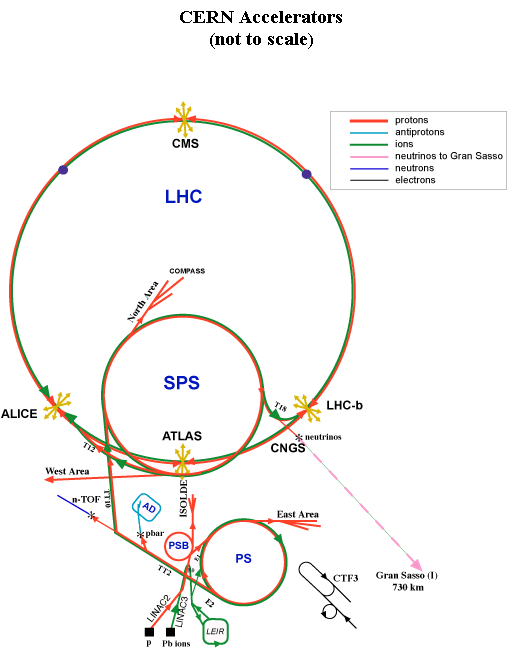
\includegraphics[height=0.8\textheight]{images/sps.png}
\end{figure} 

\column{0.5\linewidth}
\begin{itemize}
\item 1957 - Synchrocyclotron starts up
\item 1959 - Proton Synchrotron starts up
\item 1976 - Super Proton Synchrotron starts up
\item 1989 - LEP first injection
\item 1999 - Antiproton Decelerator approved
\item 2000 - LEP final shutdown
\item 2008 - LHC starts up
\end{itemize}

\end{columns}


\end{frame}

%------------------------------

\begin{frame}
\frametitle{Underground Area 1 (UA1) - detector}
\fontsize{9pt}{12}\selectfont

\begin{figure}[h]
\centering
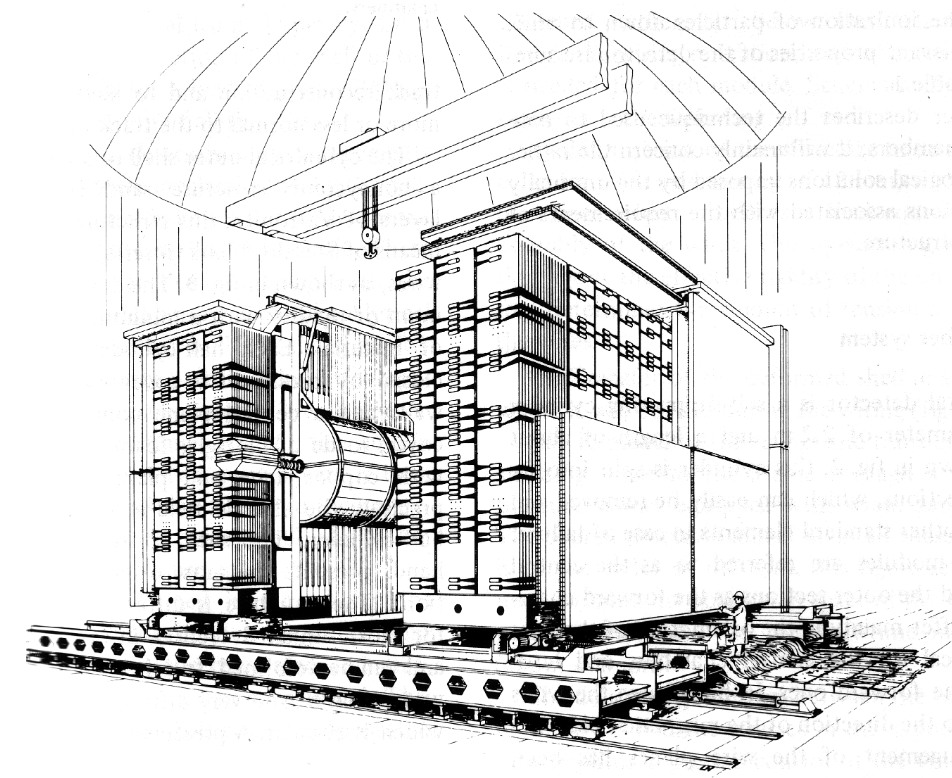
\includegraphics[height=0.75\textheight]{images/ua1-overview.png}
\end{figure}

\end{frame}

%------------------------------

\begin{frame}
\frametitle{Underground Area 1 (UA1) - detector}
\fontsize{9pt}{12}\selectfont

\begin{figure}[h]
\centering
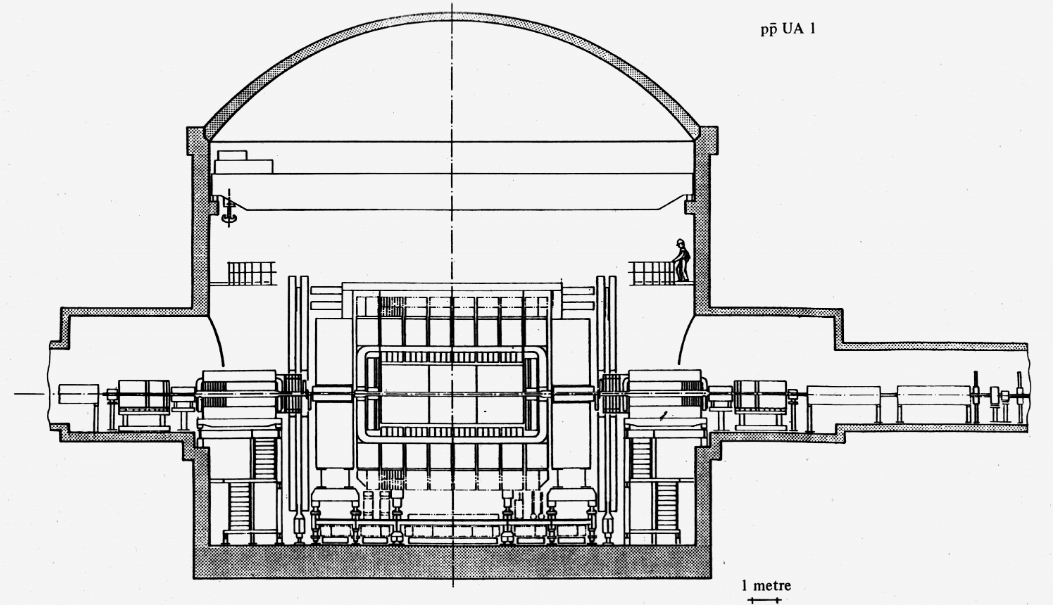
\includegraphics[height=0.7\textheight]{images/ua1-sideview.png}
\end{figure}

\end{frame}

%------------------------------

\begin{frame}
\frametitle{Underground Area 1 (UA1) - detector}
\fontsize{9pt}{12}\selectfont

\begin{itemize}
\item ran from 1981 until 1990
\item moveable detector (also UA2) custom built around SPS for $p\bar{p}$ collisions
\item could be rolled back to allow fixed-target operation of SPS
\end{itemize}

\begin{itemize}
\item transverse dipole magnet produced uniform field of 0.7T over $7\times 3.5\times 3.5\si{m^3}$
\item central detector = six-chambered cylinder, $\SI{5.8}{m}$ length, $\SI{2.3}{m}$ diameter
\item produced bubble-chamber quality pictures of each interaction
\end{itemize}


\end{frame}

%------------------------------
\begin{frame}
\frametitle{Underground Area 1 (UA1) - detector}
\fontsize{9pt}{12}\selectfont

\begin{columns}

\column{0.5\linewidth}
\begin{itemize}
\item 48 barrel EM calorimeters, called `gondolas'
\end{itemize}

\begin{figure}[h]
\centering
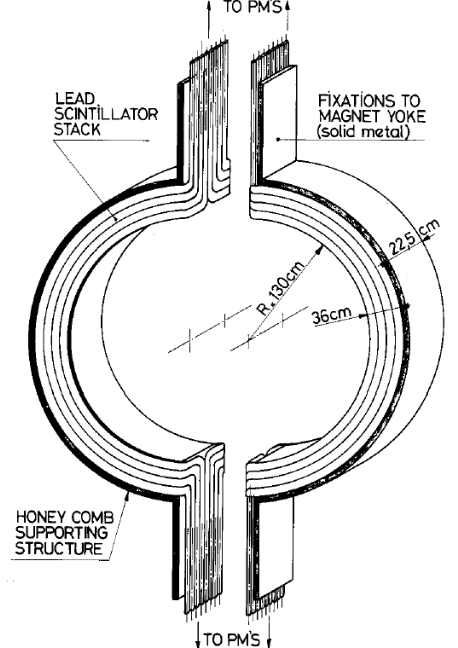
\includegraphics[height=0.65\textheight]{images/gondola.png}
\end{figure}

\column{0.5\linewidth}
\begin{itemize}
\item 64 end-cap EM calorimeters, called `bouchons'
\end{itemize}
\begin{figure}[h]
\centering
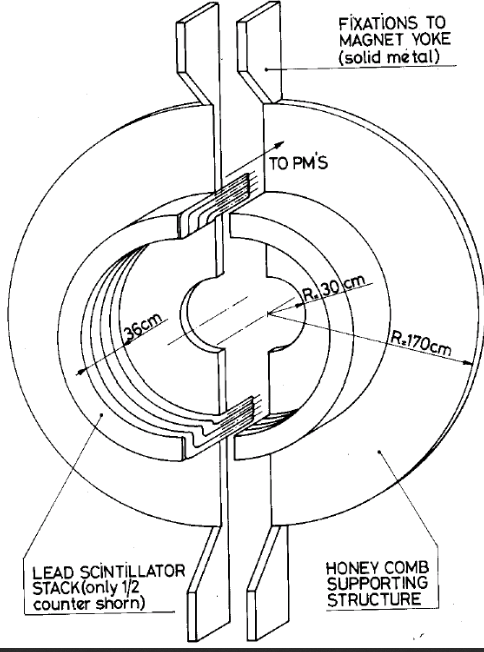
\includegraphics[height=0.65\textheight]{images/bouchon.png}
\end{figure}

\end{columns}

\end{frame}
%------------------------------

\begin{frame}
\frametitle{Underground Area 1 (UA1) - experiment}

\begin{itemize}
\item ra
\item 
\end{itemize}


\end{frame}
%------------------------------

\begin{frame}
\frametitle{Particle physics up to 1983}
\fontsize{9pt}{12}\selectfont

\begin{itemize}
\item 1897 - electron discovered
\item 1932 - positron discovered
\item 1937 - muon discovered
\item 1956 - (electron) neutrino discovered
\item 1962 - muon neutrino discovered
\item 1968 - Glashow, Weinberg and Salam formulate unified electroweak theory
\item 1969 - partons observed
\item 1975 - tau discovered
\item 1983 - ???
\end{itemize}


\end{frame}
%------------------------------

\begin{frame}
\frametitle{Particle physics up to 1983}
\fontsize{9pt}{12}\selectfont

\begin{itemize}
\item 1897 - electron discovered
\item 1932 - positron discovered
\item 1937 - muon discovered
\item 1956 - (electron) neutrino discovered
\item 1962 - muon neutrino discovered
\item 1968 - Glashow, Weinberg and Salam formulate unified electroweak theory
\item 1969 - partons observed
\item 1975 - tau discovered
\item 1983 - W and Z bosons discovered
\end{itemize}


\end{frame}
%------------------------------


\begin{frame}
\frametitle{Predictions of W mass + cross-section}



\end{frame}


%------------------------------

\begin{frame}
\frametitle{Data taking}

\begin{itemize}
\item proton and anti-protons collided at $\sqrt{s}=\SI{540}{GeV}$
\item $\SI{18}{nb^{-1}}$ data set ($\sim 10^9$ collisions), collected at UA1
\item recorded over 30 days during November and December 1982
\item triggers were used to select interesting events
\end{itemize}

\end{frame}

%------------------------------

\begin{frame}
\frametitle{Triggers}
\fontsize{9pt}{12}\selectfont

\begin{itemize}
\item four trigger conditions were required:
\begin{enumerate}
\item[(1)] at least $\SI{10}{GeV}$ is transverse energy in 2 gondolas or 2 bouchons
\item[(2)]
\end{enumerate}
\end{itemize}



\end{frame}

%------------------------------



\begin{frame}
\frametitle{Selection criteria and cuts}

\begin{itemize}
\item proton and anti-protons collided at $\sqrt{s}=\SI{540}{GeV}$
\item $\SI{14}{nb^{-1}}$ data set, collected at UA1
\end{itemize}

\end{frame}


%-------------------------------------------------------------------------------
%-------------------------------------------------------------------------------

 
\end{document}






